\section{Methods}
\begin{frame}{Particle Filter Setup}
\begin{itemize}
    \item Weighting function
        \begin{itemize}
            \item Continuous, Long Tailed, Zero-Mean 
            \item Too wide $\rightarrow$ under-sensitivity, 
                slow or no convergence
            \item Too thin $\rightarrow$ reduces robustness 
                to noise, particle deprivation
            \item For this work, $N(0, 0.005^2)$ used
        \end{itemize}
    \item Number of particles
        \begin{itemize}
            \item More particles give higher fidelity 
            \item Large Initial Particle Count (16000)
        \end{itemize}
    \item Resampling 
        \begin{itemize}
            \item Stratified Resampling can result in truncated tails 
                    on posterior
            \item Regularized Resampling can result in over smoothing and 
                    slow convergence
            \item Rarely Resampled 
        \end{itemize}
    \item Prior Distribution
\end{itemize}
\note{
\begin{itemize}
    \item Design Decisions to get this to work.
    \item Most previous works considered it possible without extremely
            high computation time.
    \item Gaussian with $0.005$ standard deviation worked because the signal
                usually swings about 1-5\%.
    \item Initially set particle count higher, dense prior, no holes
    \item After resampling region smaller
    \item Only resampled when most weights had dropped near zero, 
    \item prevents truncating the distribution, and over smoothing
    \item Lot of time optimizing prior distribution to get good results
\end{itemize}
}
\end{frame}

\begin{frame}{FMRI Noise}
\centering

Resting State Noise

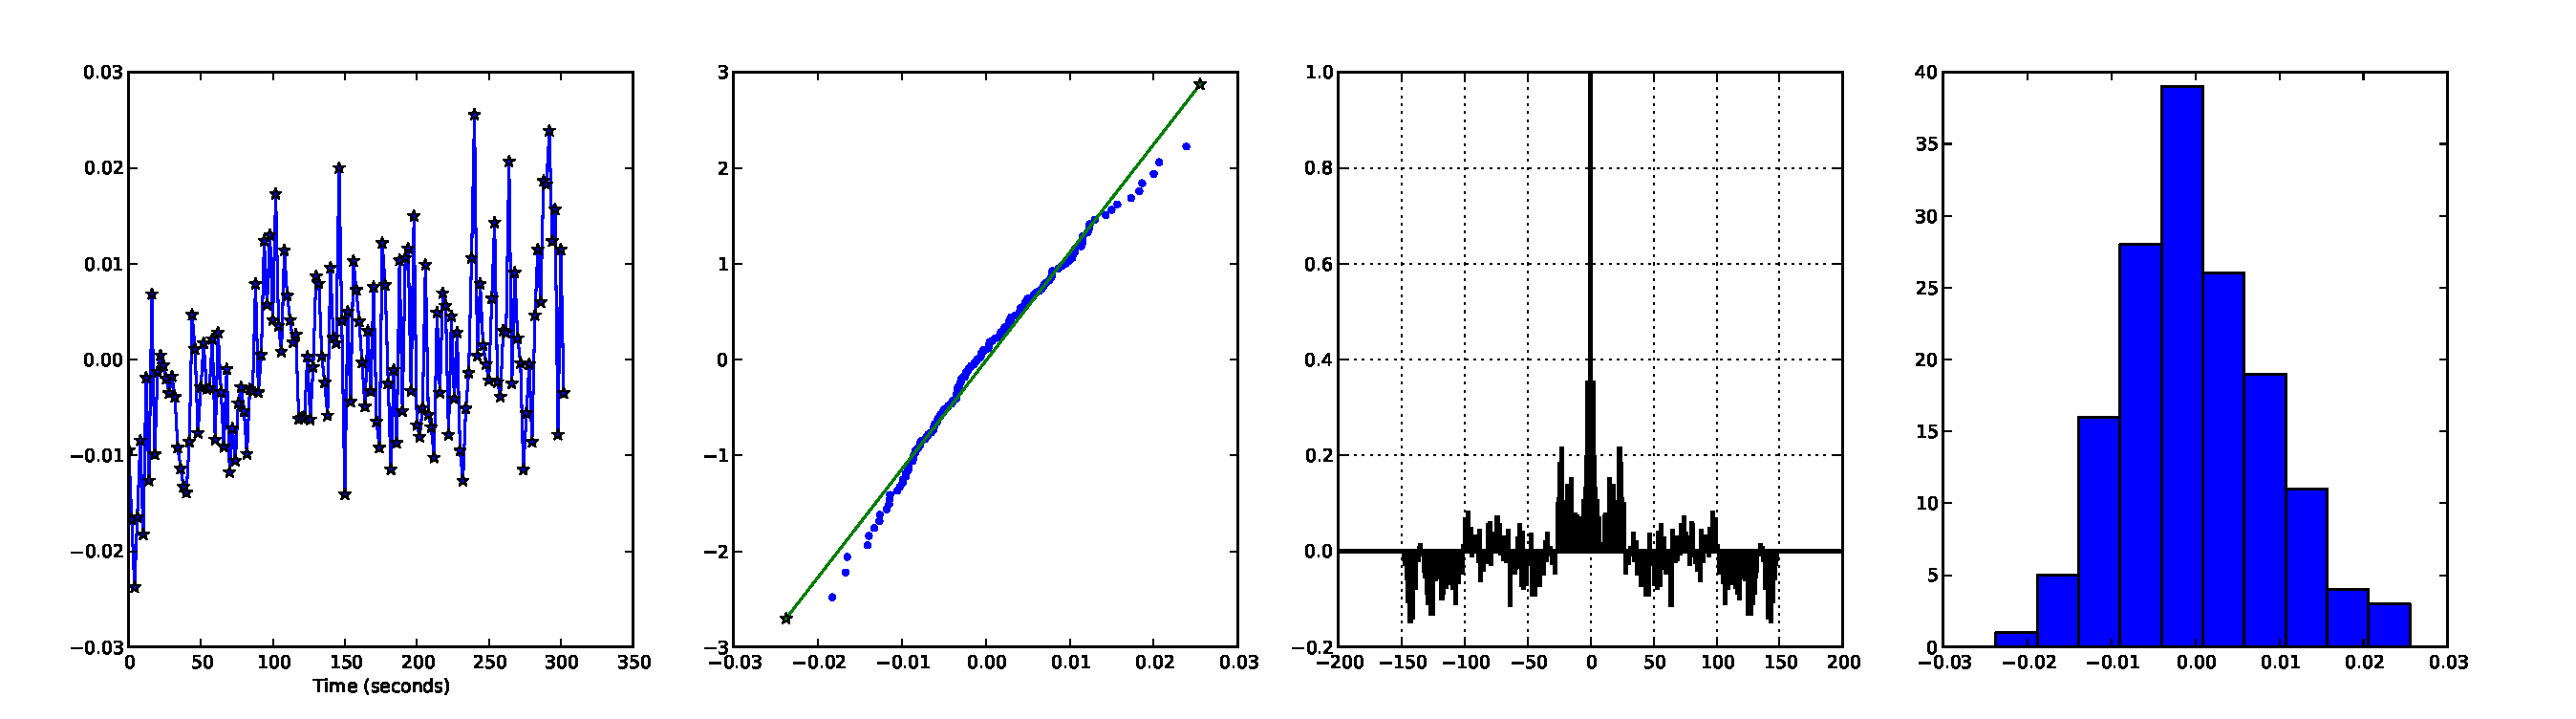
\includegraphics[trim=3cm 0cm 3cm 0cm,width=.75\textwidth]{noise2_0009_22_38_23}

Resting State Noise Steps

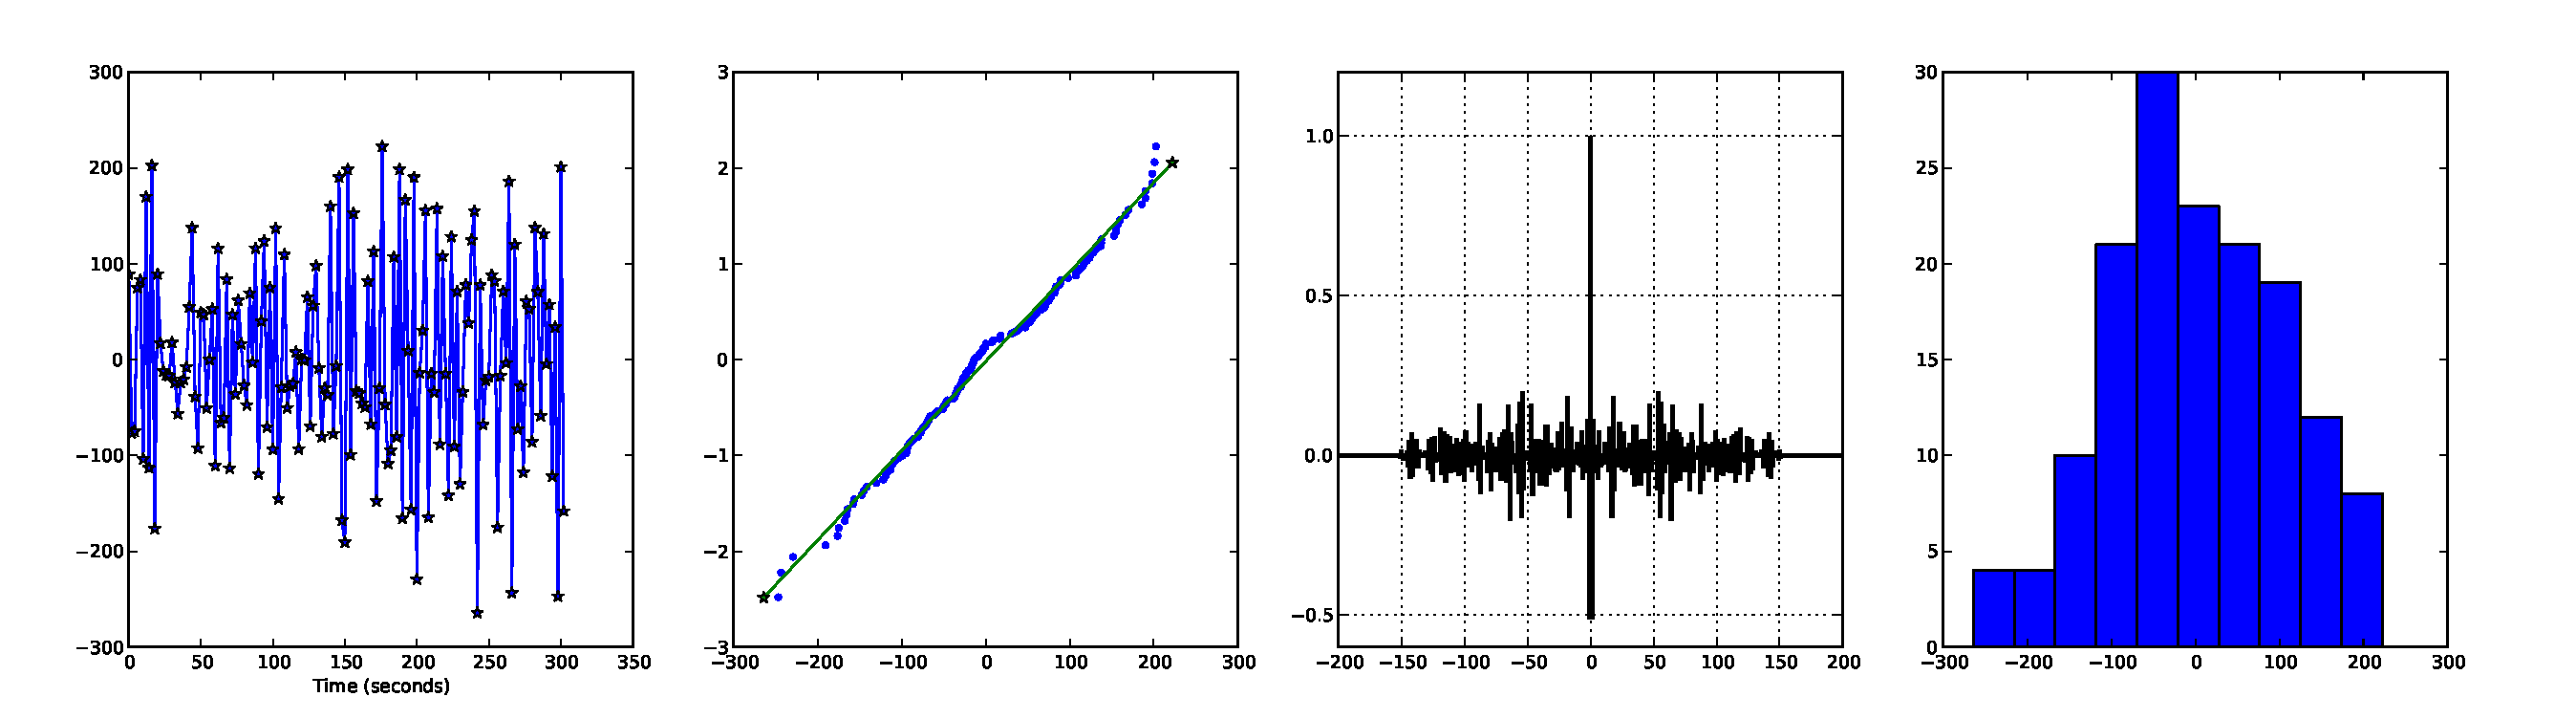
\includegraphics[trim=3cm 0cm 3cm 0cm,width=.75\textwidth]{noise2_0009d_22_38_23}

\note{
\begin{itemize}
\item Previous Works have investigated the noise extensively
\item Drift characteristic, occurs in cadavers, and after registration
\item Here I investigate the noise in resting state
\item Wiener process usually used to model drift, 
\item gaussian steps, so steps are shown on bottom
\item Left column is signal
\item Left Middle is the Q-Q plot of the samples
\begin{itemize}
\item Q-Q plot plots the quartiles of two distributions, 
\item so plot the position of the bottom 10\%, then the position of bottom 20\%
    and so on.
\end{itemize}
\item Right middle is the normalized auto-correlation
\item far right is the histogram
\end{itemize}
}
\end{frame}

\begin{frame}{Preprocessing}
  \begin{columns}
    \begin{column}{.6\textwidth}
        \begin{itemize}
            \item Drop Initial Volumes (9, $18.9$s)
            \item Realign Over Time
            \item Detrend (SPM uses $1/128 Hz$ cut off)
            \item Gaussian Smoothing (SPM Only)
            \begin{itemize}
                \item Imposes Gaussianity
                \item Increases SNR
                \item Reduces Bonferroni Correction Requirement
            \end{itemize}
        \end{itemize}
    \end{column}
    
    \begin{column}{.4\textwidth}
        \includegraphics[width=\textwidth]{preprocess}
    \end{column}
  \end{columns}
  \note{
    \begin{itemize}
        \item For SPM the default preprocessing was performed
        \item including a gaussian smoothing filter
    \end{itemize}
  }
\end{frame}

